\documentclass{IOS-Book-Article}

\usepackage{mathptmx}
\usepackage{graphicx}
\usepackage{subfigure}
\usepackage{caption}
%\usepackage{times}
%\normalfont
%\usepackage[T1]{fontenc}
%\usepackage[mtplusscr,mtbold]{mathtime}

\begin{document}
\begin{frontmatter}              % The preamble begins here.

%\pretitle{Pretitle}
\title{Parallelizing Finite Element Methods Assembly for Unstructured Meshes with D\&C}
\runningtitle{D\&C Assembly}
%\subtitle{Subtitle}

\author[A]{\fnms{Lo\"ic} \snm{Th\'ebault}%
\thanks{Corresponding Author E-mail: }},
\author[A]{\fnms{Eric} \snm{Petit}},
\author[A]{\fnms{Marc} \snm{Tchiboukdjian}},
and
\author[B]{\fnms{Quang} \snm{Dinh}}

\runningauthor{L. Th\'ebault et al.}
\address[A]{PRISM - University of Versailles, France}
\address[B]{Dassault Aviation, Saint-Cloud, France}

\begin{abstract}
Current algorithms and runtimes struggle to scale to a large number of cores and show a poor parallel efficiency on current HPC machines.
Pure MPI codes are wasting IO, memory and communication. HPC users have to explore new paradigms to make an efficient usage of the shared resources,
such as hybrid MPI+threads.
In this paper we propose and evaluate a Divide \& Conquer, D\&C, approach for the parallelization on shared memory of an unstructured mesh assembly to sparse matrix.
Our target application is an industrial CFD application from Dassault Aviation.
Our implementation is based on the versatile Cilk runtime and standard MPI.
The original Fortran code has been modified with a minimum intrusion into the original pure MPI application.
Preliminary results on the finite element assembly of the application are encouraging and show good locality and scalability characteristics.
\end{abstract}

\begin{keyword}
Divide and Conquer, Task, Cilk, Mesh Partitioning, CFD, Matrix Assembly, FEM
\end{keyword}
\end{frontmatter}

\thispagestyle{empty}
\pagestyle{empty}

\section{Introduction}
%Positionment : code MPI compare to hybrid.\\
%Problem on FEM : assembling, parallelization with shared memory non trivial.\\
%Assembling on multicore, not on GPU (most of papers are for GPUs)\\\\

Current algorithms and runtimes struggle to scale to a large number of cores and show a poor parallel efficiency on current HPC machine. 
The major effects of the core count increase are a lower memory per core, higher requirement for concurrency (thread level parallelism, instruction level parallelism, vector instructions),
higher coherency traffic and higher cost for coherency protocol.
It results in a severe challenge for performance scalability. The manycore accelerators such as the Xeon Phi exacerbate even more these issues.
HPC users have to explore new paradigms to make an efficient usage of the new resources. 

In order to mitigate the node scalability issues, users can modify their application using hybrid MPI + threads to take advantage of the full topology of the machine
and enhance the data and synchronization locality.
In this paper, we propose and evaluate a new parallelization strategy for structured problem based on the Divide and Conquer, D\&C, principle. Our implementation is based on a task based runtime,
Cilk~\cite{cilk5}. 

We demonstrate the potential of the D\&C approach on the finite element assembly step from finite element methods, FEM.
This step builds a matrix describing the linear system of equations from the mesh.
The values in the sparse matrix are the result of a reduction operation of neighbor elements.
The irregularity of the structure and the sequentialization of the reduction are challenging to achieve an efficient parallelization.
For multicores, except the state of the art coloring approaches, there are few recent works published on parallelizing FEM assembly codes.
In the manycore context, new algorithms are design for GPUs~\cite{cecka2011assembly,CPUGPUasm}, but can not be efficiently applied to shared memory systems of multicores.

We apply our D\&C strategy to parallelize the finite element assembly of an industrial fluid dynamics code from Dassault Aviation.
This code computes the effect of mesh deformation to optimize airplane structure.
Our results outperform the original pure MPI implementation and the coloring method for shared memory parallelization and vectorization.
\\\\
The paper outline is the following:
\begin{itemize}
\item Section 2 presents the finite element assembly in applications using the coloring approach and our D\&C proposal using Cilk and MPI.
\item Section 3 presents related works on assembly of finite elements and different parallelization strategies.
\item Section 4 presents the experimental setups and results of the FEM assembly parallelization of a Dassault Aviation application, called DEFMESH.
\item Section 5 concludes and presents our future works.
\end{itemize}

\section{FEM Assembly}
%The process alterate the mesh geometry and be conservative of the mesh topology.  We have to work on a very unstructured mesh. Therefore, load balancing and interface
%computation prevent us to use geometrical domain decomposition.
%We use METIS~\cite{Metis} to do a topological domain decomposition that will not vary with the mesh deformation.
%The application iterates over three basic steps:
%\begin{itemize}
%\item Edge matrix assembly to CSR storage from the mesh coordinate array. This step potentially needs MPI communication in the case of using the elastic version.
%Explain in section ...
%\item Solve ... ??? what?
%\item Update the mesh coordinate and value, exchange the halo with other MPI rank.
%\end{itemize}

Finite element assembly is common in most of scientific applications using finite element methods.
A simple FEM assembly illustration of a 2D regular mesh is presented in figure~\ref{fig:2Dasm} with the associated sparse matrix.
The values of the edges are the reduction of neighbor element contribution. In figure~\ref{fig:2Dasm}, $(N1,N2) = E1 + E2$.
The non-zero values of the matrix corresponds to the edges of the mesh. This matrix is sparse and symmetrical, thus we store only the lower triangular non-zero values.
In 3D, the number of neighbor elements can be arbitrary large.

To create parallelism, we must build independent domains to compute in parallel and synchronize between them to handle shared edges.
We consider two different approaches, a state-of-the-art coloring approach and our proposal of D\&C strategy based on a topological recursive bisection.
\begin{figure}[htp]
 \centering
 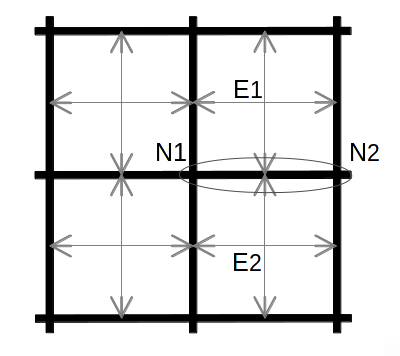
\includegraphics[scale=0.2]{2D_asm.png}
 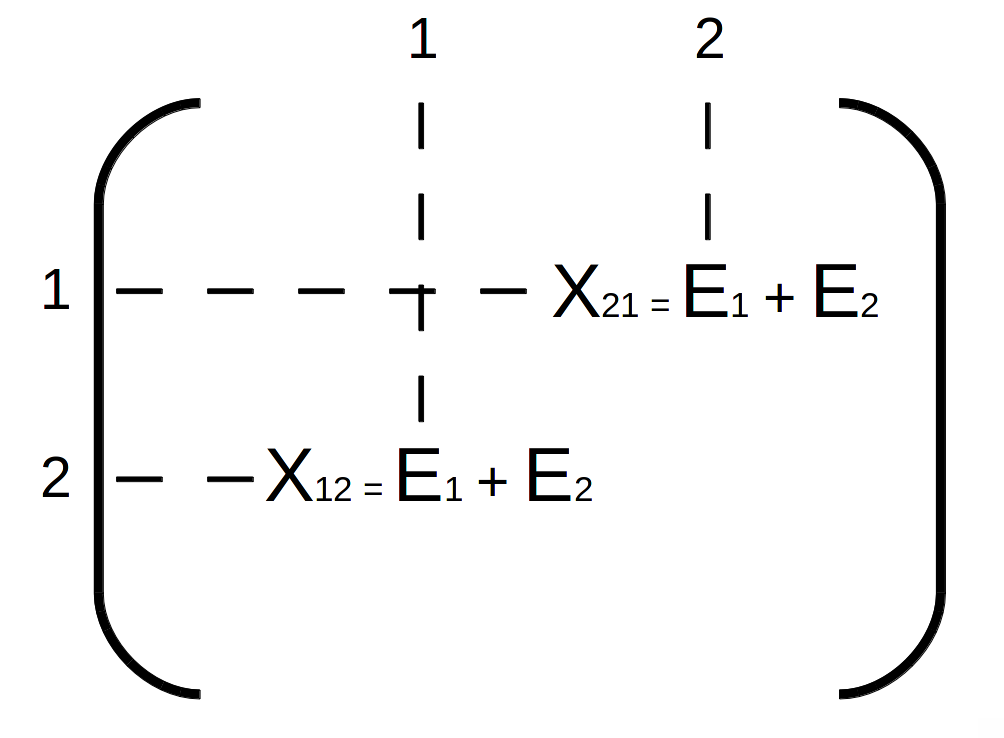
\includegraphics[scale=0.12]{Matrix_asm.png}
 \caption{2D FEM assembly example}
 \label{fig:2Dasm}
\end{figure}

\subsection{Coloring}
\label{sec:col}
Coloring avoids race conditions by assigning a different color to the elements sharing an edge.
It was originally targeting vector machines because elements of a same color do not contribute to the same edges.
Determining a minimal coloring is NP-complete, but creating an efficient coloring with a larger number of colors using heuristic is well-known in litterature~\cite{CPUfe}.
A pseudo-code and a simple 2D coloring example are given in figure~\ref{fig:colApp}.
~\\~\\~\\
{
\begin{minipage}[tp]{0.34\textwidth}
	%\centering
	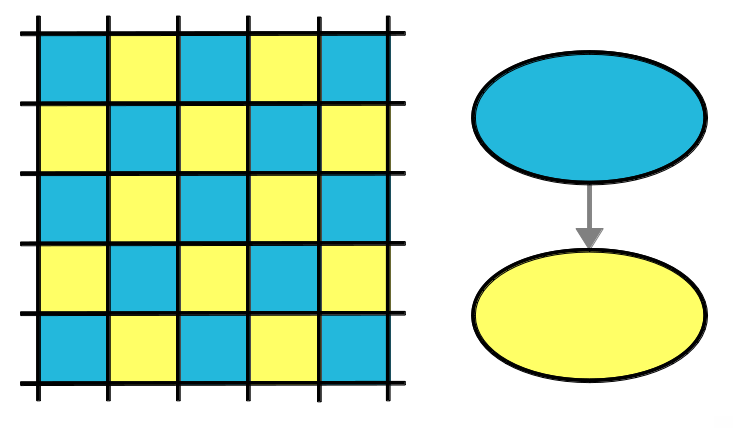
\includegraphics[scale=0.15]{Coloring_approach.png}
\end{minipage}
\begin{minipage}[tp]{0.55\textwidth}
 		\small
 		\begin{verbatim}
			NodeToElem=node2element(ElemToNode)
			ElemToElem=element2element(NodeToElem)
			ElemToColor=element2color(ElemToElem)
			ColorToElem=color2element(ElemToColor)

			For each color C in colors
    				Parallel_For all elements E in C
        					compute_element_contribution(c)
 		\end{verbatim}
 \end{minipage}	
 \captionof{figure}{\label{fig:colApp} The coloring approach}
 }
 ~\\
Despite coloring is an efficient approach for vectorial machines, it is not well suited for current shered memory parallel architectures.
Sorting the elements by color improves the spatial locality and enables vectorization.
However, there is only one update per edge and per color. Furthermore each color covers the whole domain.
Thus for large domains, there will be no edge locality in cache between colors.

\subsection{Divide \& Conquer}
%D\&C, approach on  unstructured meshes
%%
%The D\&C approach is particularly interesting for its ability to scale naturally to an increasing number of node thanks to its architecture oblivious concept.
%Each leaves is responsible of its own data and there is a very minimal amount of sharing, avoiding costly locks and coherency protocols. 

The main idea of the D\&C approach for shared memory parallelization is to enable task level parallelism while preserving good data locality and minimizing synchronization cost.
When the size of the domain increases, we increase the number of Cilk tasks and threads instead of increasing the number of MPI domains and the amount of communication.
This way, we take the benefit of the machine topology and most of communication are replaced by data sharing.

The rational is to divide recursively the work in two or more independent tasks and synchronize these tasks locally. This recursive approach has many advantages.
First the recursive sharing naturally exposes high concurrency. As long as the application is large enough, it is possible to produce a deeper recursive tree to get more concurrency and 
therefore match the higher requirement of manycore systems. Furthermore, synchronizations are local: only nodes of a same parent in the recursive tree need to be synchronized.
Finally, D\&C approach improves the data locality by reordering the data. 

On a small number of cores, the scalability of the D\&C parallelization is expected to be equivalent to the pure MPI.
However, for a larger number of cores, D\&C should continue scaling while pure MPI should not.
In any case the code will benefit from the higher locality and reuse of elements in the D\&C version and all the versions using the reordering should outperform the original code.

This approach consists of two parts described in following subsections.
First part is the recursive decomposition of each MPI domain and second part is the recursive execution of the FEM assembly step using Cilk.

\subsubsection{Recursive Bisection}
\label{sec:DCrec}
D\&C is based on a topological recursive bisection of the mesh.
As illustrated in figure~\ref{fig:DCapp}, the left and right sub-domains created by these bisections do not share any element and thus, can be executed in parallel.
However, the separator elements in the middle have nodes in both sides and must be processed after left and right sub-domains.

The load-balancing between the sub-domains is important since it influences the depth of the recursive tree.
A balanced tree will minimize the maximum depth and thus the number of synchronization on the critical path.
Therefore, it is important to use a good partitioner to build equal sub-domains. In this study, we use the METIS graph partitioner~\cite{Metis}.

In order to increase the data locality, we permute node and element arrays.
Indeed, nodes and elements can be consecutive in memory inside each sub-domain, improving intra-task locality.
Secondly, since the tasks distribution is following the recursive domain decomposition, we store neighbor sub-domains and associated separator contiguously
to improve locality between tasks.
These permutations are applied to all MPI domains, therefore we renumber the nodes on the frontier so that exchanged data is consistent.
\begin{figure}[htp]
 \centering
 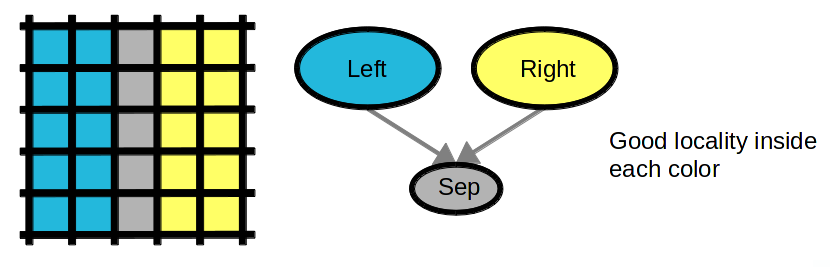
\includegraphics[scale=0.17]{DC_approach.png}
 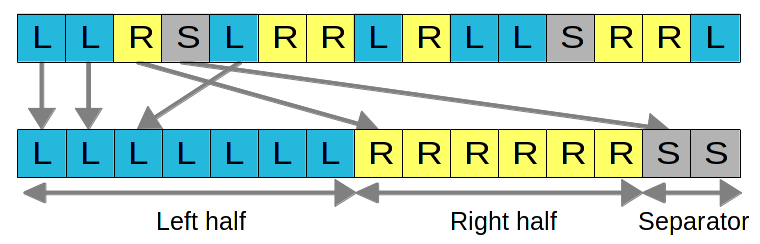
\includegraphics[scale=0.21]{Data_permutations.png}
 \caption{D\&C approach}
 \label{fig:DCapp}
\end{figure}

The proposed approach is then applied recursively to all sub-domains, providing a large amount of parallelism.
As illustrated in figure~\ref{fig:DCrec}, each leaf of the resulting tree is associated with an independent Cilk task which executes the FEM assembly process on its sub-domain.
In order to optimize the locality with permutations without multiplying tasks, it is possible to stop the recursion before reaching the leaves.
To do so, the tasks execute in one block the left, right and separator domains contiguously stored in memory.

The partitionment is topological: cuts are done on edges rather than on geometrical coordinates.
This allows to compute sub-domains only one time for a mesh, and it is independent from the rest of the computation. Therefore, this partition is precomputed and stored with the mesh.
During the run, the application needs only to apply the precomputed permutations before executing the recursive FEM assembly.
\begin{figure}[htp]
 \centering
 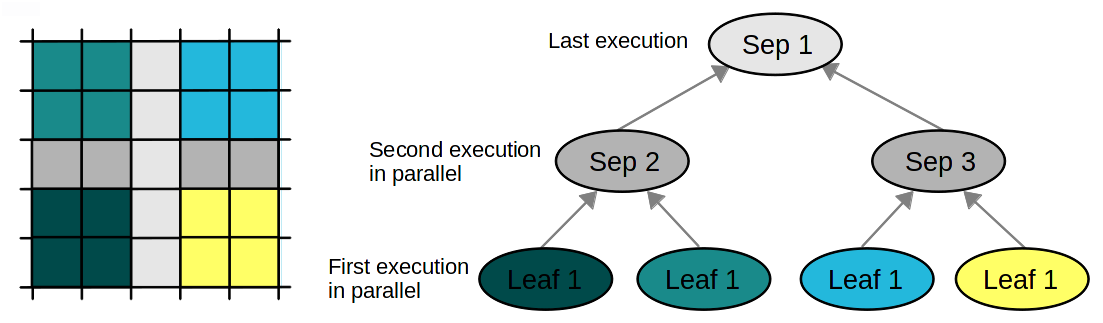
\includegraphics[scale=0.25]{DC_recursion.png}
 \caption{D\&C recursive execution}
 \label{fig:DCrec}
\end{figure}

\subsubsection{Cilk Implementation}
Cilk~\cite{cilk5} is a task based runtime originally developed by Frigo, Leiserson and Randal at MIT and now supported by Intel.
It allows users to \emph{spawn} and \emph{sync} many parallel tasks.
All these tasks are organised in queues and executed by \emph{worker} threads.
For load balancing, Cilk runtime uses a work-stealing scheduler. When a \emph{worker} completes its queue, it can steal additional tasks from slower \emph{workers}.

Once the tree like the one shown in figure~\ref{fig:DCrec} is constructed, the Cilk implementation is straightforward.
Until the recursion has not reached a leaf (domain size condition), left and right sub-domains of each node are split in two tasks and executed in parallel.
These tasks have to complete before launching the separator computation. 
When the recursion reaches the leaves, the original sequential FEM assembly routine is executed on their sub-domains, see figure~\ref{fig:DCcode}.

When all elements are accessed in a regular loop, there is no need to use a recursive task tree.
In this case, similarly to OpenMP, Cilk provides an easy way to parallelize loops using the \emph{cilk\_for} keyword.
By substituting the original \emph{for} with the \emph{cilk\_for} keyword, iterations of the loop are split recursively in several parallel tasks.
For the DEFMESH application, we observe a better scalability with the \emph{cilk\_for} than with \emph{OpenMP parallel for} pragma.
\begin{figure}[htp]
\small
 \begin{verbatim}
function compute (sub-domain) 
    if Node is not a leaf
        spawn compute (sub-domain.left)
        compute (sub-domain.right)
        synchronize
        compute (sub-domain.sep)
    else
        FEM_assembly (sub-domain)
end        
 \end{verbatim}
 \caption{D\&C assembly pseudo-code}
 \label{fig:DCcode}
\end{figure}

\section{Related Works}
Many choices are available to complete FEM assembly in parallel.
All methods have their advantages and their limitations, depending for instance on the target architecture or the mesh size.
Recent studies~\cite{cecka2011assembly,CPUGPUasm} investigate different ways to compute FEM assembly on CPUs and GPUs.
A first method presented in~\cite{cecka2011assembly} consists in creating parallelism between all the non-zero entries of the system of equations.
This method has a very fine grain thread parallelism and thus can be applied only to GPUs.
First, they store contributions from all elements in the global or local memory in parallel and then reduce in parallel these contributions to compute the non-zero values.
By arranging the data layout, this method can provide good performance on GPUs.
However, this method can suffer from bad load balancing since the number of neighbor elements to compute non-zero values can vary.
Moreover, the amount of local copies grows quickly and thus the approach is limited to relatively small test cases.
Another variant consists in using one thread for the whole FEM assembly step of one non-zero value at a time, but this approach leads to redundant computations of element contributions.

A second method~\cite{cecka2011assembly} consists in assembling by mesh element. One thread is responsible for the whole FEM assembly step of one element at a time.
It can be applied to both GPUs and CPUs.
A coloring approach~\cite{CUDAfe,CPUfe} can be used to launch several threads in parallel on independent elements.
This way each thread has a good load balancing per color. The load balancing between colors has no influence since they are sequentialized.
However, bad data locality can cause poor performance as explained is section~\ref{sec:col}.

Divide and Conquer paradigm and recursion in general has been already explored for a long time for parallel algorithm~\cite{div}.
M. Martone et al.~\cite{RSBasm} describe a matrix assembly approach for recursive sparse blocks (RSB) matrix on CPUs.
Despite this format can provide good results in solver algorithms~\cite{RSBsolver}, according to authors results, FEM assembly on RSB matrix is memory-bandwidth bound~\cite{RSBasm}.
In 2008, Dongarra et al.~\cite{Dongarra} evaluated an asynchronous task based parallelism approach for well-known factorization algorithms and compared it to traditional fork-join approach.
A recent investigation on hybrid programmation integrating task base parallelism in MPI processes have been made~\cite{MPIhybid}.
The experiments done on a 1024 nodes cluster result in significant speed-up on several micro-benchmarks and strong scaling applications compared to pure MPI.

\section{Experiments}
To validate our approach, we apply the D\&C algorithm using Cilk and MPI to the FEM assembly step of an application from Dassault Aviation called DEFMESH.
We compare our results to the pure MPI original version of the FEM assembly step and also to the MPI + OpenMP version using the coloring approach.

\subsection{Dassault Aviation DEFMESH Application}
The DEFMESH application is a computational fluid dynamics (CFD) code based on a finite element method (FEM).
This volume mesh deformer, is an important numerical module in Dassault Aviation aerodynamic optimization environment.
It is also used in other simulations which may include surface variations of larger magnitude, such as in aero-elastic interactions or dynamics of moving bodies.

DEFMESH implements a three-dimensional elasticity-like system of equations from given surface data.
These equations are solved by two different alogorithms.
First one is a linear algorithm used when the magnitude of the surface data is small, the equations can be linearized into a system of linear equations with a symmetric definite positive matrix.
Second one is a non linear algorithm where surface data of large magnitude are cut in a succession of small increments.
The original equations are solved as a non-linear succession of linearized sub-problems, consisting of systems of linear equations, each with a symmetric definite positive matrix.
The systems of linear equations, with a symmetric definite positive matrix, are solved by a standard conjugate gradient (CG) algorithm.

DEFMESH implements two options for the definition of the elasticity-like operator for its system of volume equations.
The Laplacian operator, which calls 3 times the CG algorithm at each linearized step. Each call computes the solution of a scalar system of linear equations.
Secondly, the Elasticity operator, where the full 3D linear elasticity operator is implemented.
It couples the 3 mesh coordinates, thus at each linearized step, the CG algorithm has to solve a 3 by 3 system of linear equations.
The “Elasticity operator” permits mesh deformations of greater magnitude and smoother deformed meshes than the “Laplacian operator”.

DEFMESH main kernel is decomposed in three steps.
First one is the FEM assembly, where mesh data are gathered into a CSR structure.
Second step is the solver which works on this CSR structure and computes optimal displacements.
Final step is the update of mesh coordinates using previously computed deformations.

We performed our experiments on an unstructured mesh from Dassault Aviation, called EIB and illustrated in the figure~\ref{fig:reservoir}.
It is composed of 6 346 108 elements and 1 079 758 nodes and it represents the displacements of a fuel tank along an airplane fuselage.
\begin{figure}[htp]
 \centering
 \subfigure[]{\label{fig:EIB3D}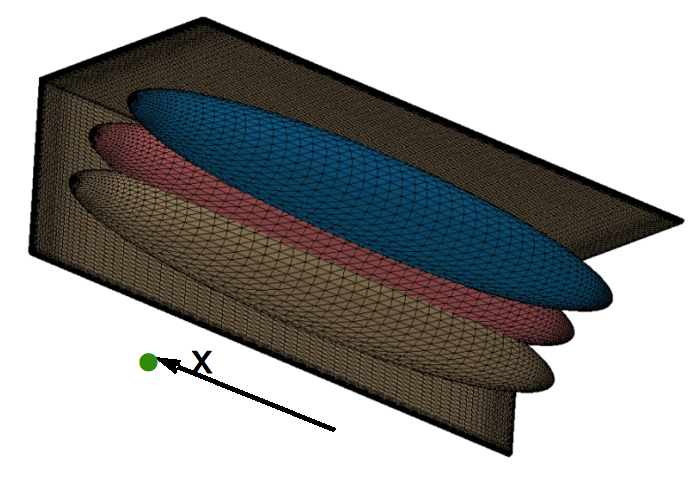
\includegraphics[width=0.49\textwidth]{reservoir_3D.png}}
 \subfigure[]{\label{fig:EIB_proj}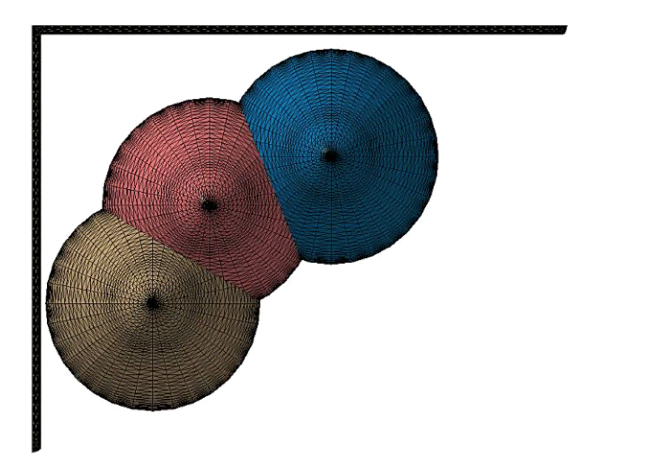
\includegraphics[width=0.49\textwidth]{reservoir_projection.png}}
 \subfigure[]{\label{fig:EIB_high}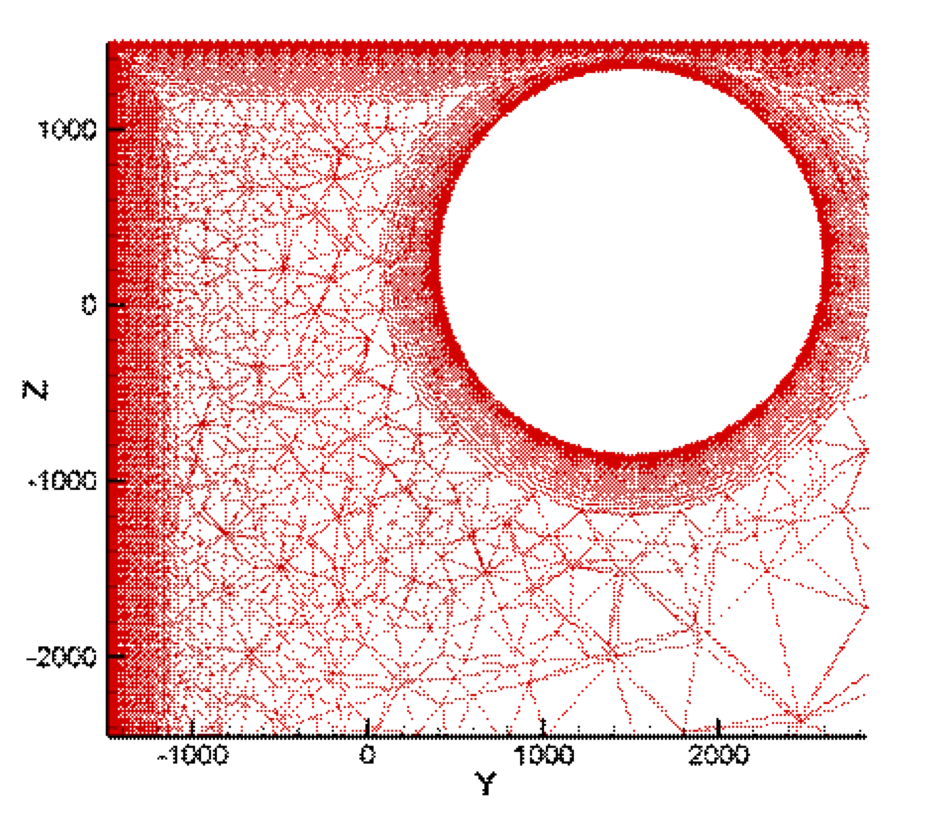
\includegraphics[width=0.32\textwidth]{reservoir_haut.png}}
 \subfigure[]{\label{fig:EIB_middle}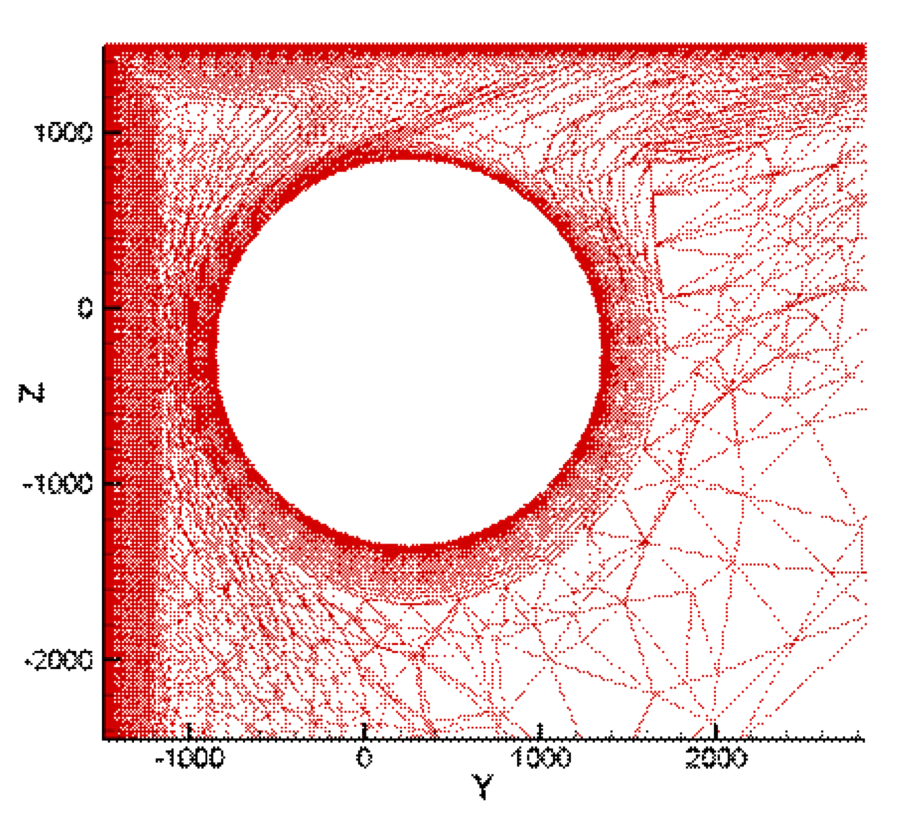
\includegraphics[width=0.32\textwidth]{reservoir_milieu.png}}
 \subfigure[]{\label{fig:EIB_middle}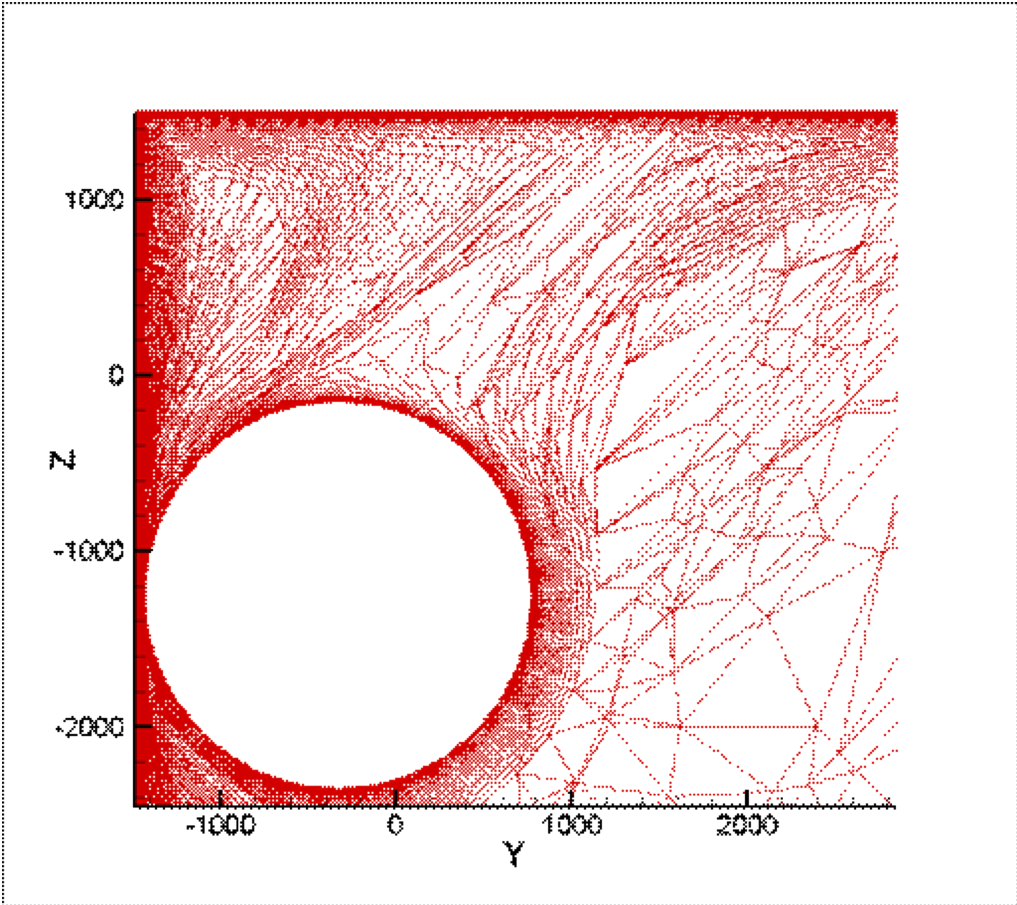
\includegraphics[width=0.32\textwidth]{reservoir_bas.png}}
 \caption{EIB fuel tank position optimization test case}
 \label{fig:reservoir}
\end{figure}

\subsection{Experimental Setup}
In the following experiments, we compare two versions of the DEFMESH application: the original one from Dassault Aviation called $Ref$ and the new Divide \& Conquer version called $D\&C$.
The original version uses MPI between the different blocks of the mesh and OpenMP to parallelize the sparse matrix-vector loop of the solver.
The D\&C version uses the recursive partitioning of each block of the mesh.
In addition to MPI and OpenMP, this version also exploits a Cilk task parallelism in the FEM assembly.
We also compare our results to the coloring implementation of the FEM assembly, using OpenMP.

For each of these versions, we consider the Laplacian and elasticity variants of DEFMESH.
For both of them, the application runs in 50 steps of resolution and the measures correspond to the average time of one iteration.
In all cases we measure the FEM assembly step, where the D\&C approach has been applied.
We also measure the solver to estimate the impact of the data permutations on the rest of the code.

We present the results both in terms of execution times and of parallel efficiency.
In all the graphics, the \emph{x} axis represents the number of cores. It corresponds to the number of MPI processes multiplied by the number of threads.
In figures presenting execution time, the \emph{y} axis corresponds to RDTSC cycles for the FEM assembly and to \texttt{MPI\_Wtime} for the solver.
Concerning efficiency, the \emph{y} axis represents the parallel efficiency given by the following formula:
$E_{P} = \frac{T_{S}}{P*T_{P}}$, where $E_{P}$ is the efficiency on $P$ processor, $T_{S}$ the sequential time, and $T_{P}$ the time on $P$ processors.

For each figure, we use 1, 4, 8 and 12 MPI processes and 1 to 12 threads, OpenMP or Cilk, while the multiplication of MPI processes per thread is lower or equal to 12.
This corresponds to the number of cores available. In all cases, the number of Cilk threads used in the FEM assembly is equal to the number of OpenMP threads used in the solver.
We also varied the number of METIS partitions and the number of Cilk tasks, but we have not observed significant changes in the results.
According to the Cilk documentations, 10 tasks per core is appropriate. Therefore we use 128 Cilk tasks, which is also enough to fit in cache.
We cut MPI domains in 512 partitions to improve locality.

The OpenMP affinity is set to scatter and Cilk threads are not pinned.
We perform these experiments on twelve cores grouped in two sockets of 6 cores Intel® Xeon® X5650 clocked at 2.67 GHz.
Each core has its own L1 (32KB) and L2 (256KB) caches and a shared L3 cache of 12MB. The main memory is divided in two NUMA nodes of 16GB.

\subsection{Results}
The following sections present our measurement for the elastic and Laplacian version for the FEM assembly. 

NOTE TO THE REVIEWERS: The experiments on coloring are in progress and will be included in the final version of the paper.

\subsubsection{Assembly}
As we can see in figures~\ref{fig:asmCurvesA} and~\ref{fig:asmCurvesC}, the D\&C approach is slower than pure MPI, especially when we increase the number of cores.
This is due to the remaining sequential part of the D\&C code and the low intensity work in the Laplacian version.
Indeed, separator elements are not parallelized and can represent an important proportion of the computation.
According to the Amdahl law, by increasing the number of cores, the proportion of the sequential part increases. This is confirmed on figure~\ref{fig:asmCurvesC} showing the parallel efficiency.

In the elasticity variant, illustrated in figures~\ref{fig:asmCurvesB} and~\ref{fig:asmCurvesD}, the D\&C approach becomes equivalent to pure MPI.
Since the amount of work of the FEM assembly step is bigger than in the laplacian variant, the proportion of the sequential computation, including the separators, is lower.
In this case the scalability improves. Futhermore, contrary to the pure MPI version, the data always fits in L2 cache with the D\&C version.
Unlike the original version that makes irregular accesses to the cells of the matrix, the D\&C version works on matrix cells packed contiguously in small sub-matrix corresponding to the Cilk tasks.
For any problem size, with D\&C, we can increase the number of partitions such that the tasks working-set will always fit in cache.

To conclude, these first results are encouraging and we can reasonably expect to match the ideal scaling when the separators will be parallelized.

\begin{figure}[htp]
 \centering
 \subfigure[Laplacian execution time]{\label{fig:asmCurvesA}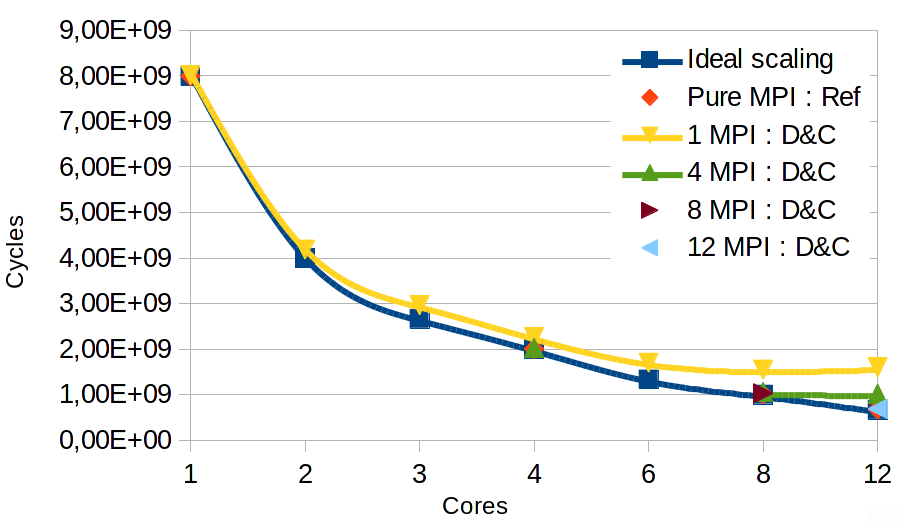
\includegraphics[width=0.49\textwidth]{Laplacian_asm_time.png}}
  \subfigure[Laplacian parallel efficiency]{\label{fig:asmCurvesC}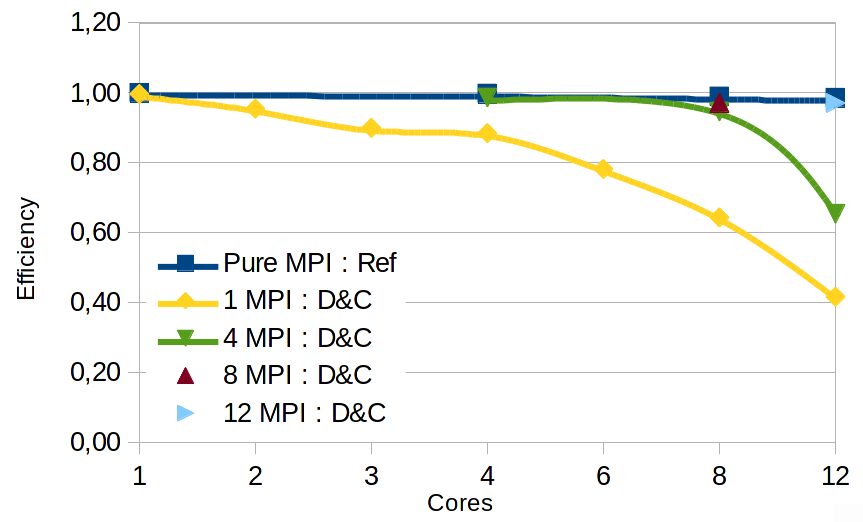
\includegraphics[width=0.49\textwidth]{Laplacian_asm_efficiency.png}}
 \subfigure[Elasticity execution time]{\label{fig:asmCurvesB}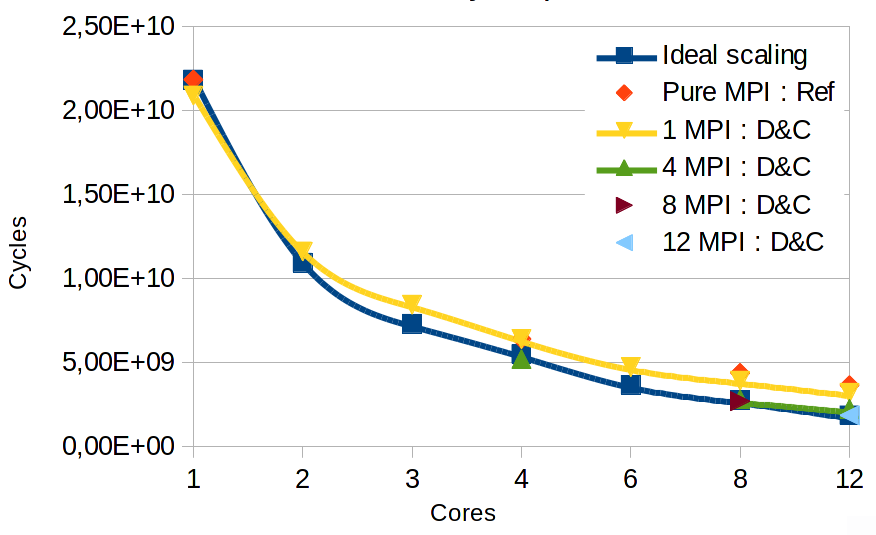
\includegraphics[width=0.49\textwidth]{Elasticity_asm_time.png}}
 \subfigure[Elasticity parallel efficiency]{\label{fig:asmCurvesD}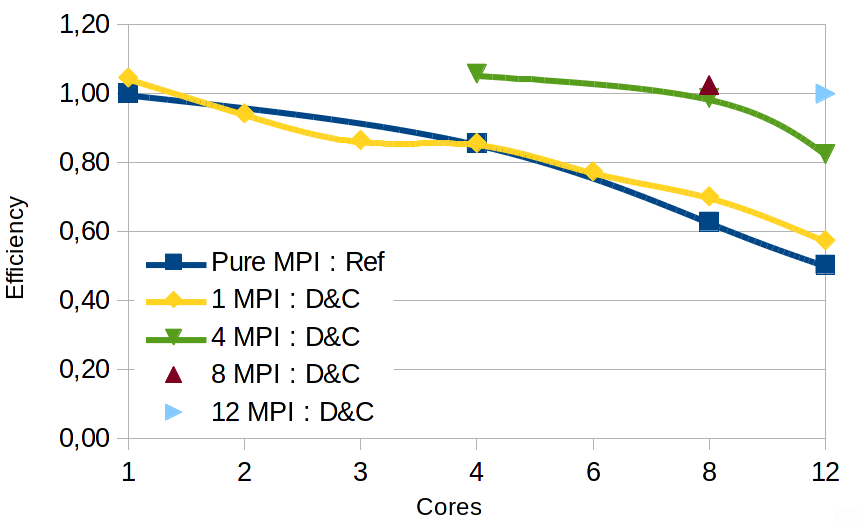
\includegraphics[width=0.49\textwidth]{Elasticity_asm_efficiency.png}}
 \caption{Assembly measures}
 \label{fig:asmCurves}
\end{figure}

\subsubsection{Solver}
Despite we did not modify the solver part, we observe in figure~\ref{fig:solCurves} approximately 6\% speed-up for the D\&C version compared to the reference version.
This gain is due to the better data locality enabled by the permutations explained in section~\ref{sec:DCrec}.
To show the impact of locality, we randomly permute the data and observe a degradation of the performance.
The result shows that the initial data already expose good locality.
Moreover, when measuring the L3 cache misses occurring in the solver for the original version and for the D\&C permutted version, they are 23\% lower with D\&C.

\begin{figure}[htp]
 \centering
 \subfigure[Laplacian]{\label{fig:solCurvesA}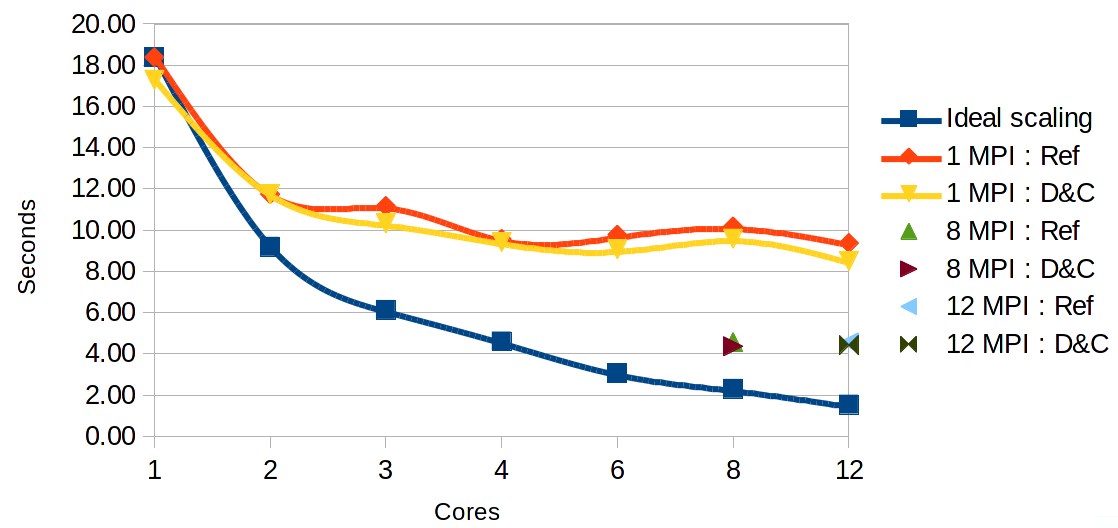
\includegraphics[scale=0.158]{Laplacian_solver_time.png}}
 \subfigure[Elasticity]{\label{fig:solCurvesB}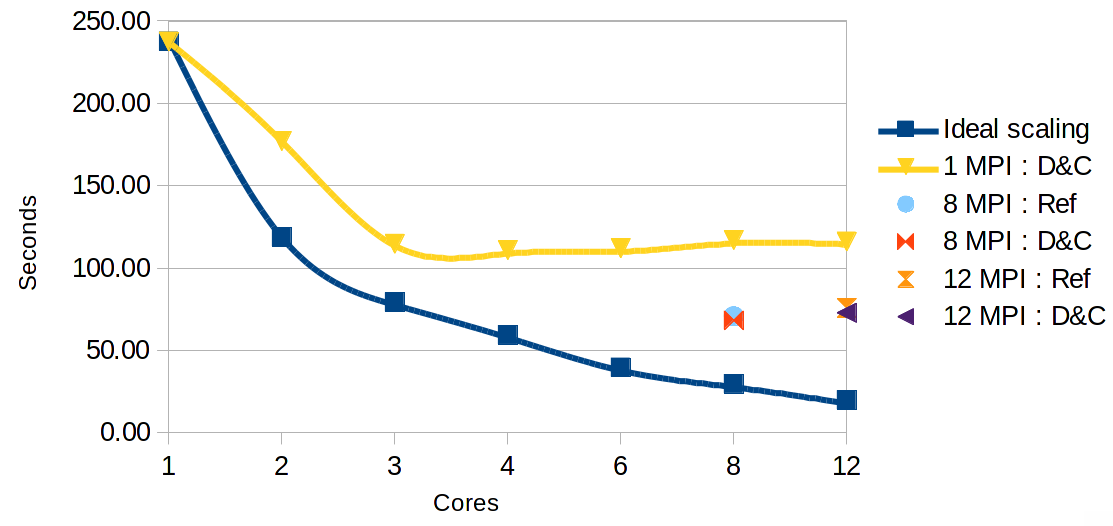
\includegraphics[scale=0.154]{Elasticity_solver_time.png}}
 \caption{Solver execution time}
 \label{fig:solCurves}
\end{figure}

\section{Conclusion and Future Work}
FEM assembly is the first step of many applications, such as seismic simulation, metal forming, or crash test simulations.
Depending on the application, the FEM assembly can cover more than 80\% of the execution time.
In the Dassault Aviation DEFMESH application, our current implementation is already faster than the pure MPI original version and overpasses in performance and scalability the state-of-the-art coloring approach.

Even without exploiting the thread level parallelism, the D\&C approach  significantly improves the locality, the scalability, and the execution time.
The pure MPI version with D\&C has a perfect strong scaling for our experimental setup.

As a future work, we plan to parallelize the separator in the D\&C FEM assembly and experiment on a larger number of cores.
We strongly believe that our approach will provide good performances on new manycores such as Xeon Phi.
Extension will focus on D\&C friendly data structure definition and apply D\&C on other parts of the FEM application. 
%We are also considering a hybrid approach using coloring inside each D\&C sub-domains in order to enable vectorization.
\bibliographystyle{unsrt}
\bibliography{dc_bib}

\end{document}